% Created 2015-06-06 sam. 19:44
\documentclass[11pt,xcolor=dvipsnames,presentation]{beamer}
\usepackage[utf8]{inputenc}
\usepackage[T1]{fontenc}
\usepackage{fixltx2e}
\usepackage{graphicx}
\usepackage{longtable}
\usepackage{float}
\usepackage{wrapfig}
\usepackage{rotating}
\usepackage[normalem]{ulem}
\usepackage{amsmath}
\usepackage{textcomp}
\usepackage{marvosym}
\usepackage{wasysym}
\usepackage{amssymb}
\usepackage{hyperref}
\tolerance=1000
\usedescriptionitemofwidthas{bl}
\usepackage[T1]{fontenc}
\usepackage[utf8]{inputenc}
\usepackage[american, english]{babel}
\usepackage{ifthen,figlatex,amsmath,amstext,gensymb,amssymb}
\usepackage{boxedminipage,xspace,multicol}
%%%%%%%%% Begin of Beamer Layout %%%%%%%%%%%%%
\ProcessOptionsBeamer
\usecolortheme{whale}
\usecolortheme[named=BrickRed]{structure}
\useinnertheme{rounded}
\useoutertheme{infolines}
\setbeamertemplate{footline}[frame number]
\setbeamertemplate{headline}[default]
\setbeamertemplate{navigation symbols}{}
\defbeamertemplate*{headline}{info theme}{}
\defbeamertemplate*{footline}{info theme}{\leavevmode%
\hbox{%
\begin{beamercolorbox}[wd=.2\paperwidth,ht=2.25ex,dp=1ex,center]{author in head/foot}%
\usebeamerfont{author in head/foot}\insertshortauthor
\end{beamercolorbox}%
\begin{beamercolorbox}[wd=.71\paperwidth,ht=2.25ex,dp=1ex,center]{title in head/foot}%
\usebeamerfont{title in head/foot}\insertsectionhead
\end{beamercolorbox}%
\begin{beamercolorbox}[wd=.09\paperwidth,ht=2.25ex,dp=1ex,right]{section in head/foot}%
\usebeamerfont{section in head/foot}\insertframenumber{}~/~\inserttotalframenumber\hspace*{2ex}
\end{beamercolorbox}
}\vskip0pt}
\setbeamertemplate{footline}[info theme]
%%%%%%%%% End of Beamer Layout %%%%%%%%%%%%%
\usepackage{verbments}
\usepackage{xcolor}
\usepackage{color}
\usepackage{url} \urlstyle{sf}
\let\alert=\structure % to make sure the org * * works of tools
\usetheme{default}
\author{Steven QUINITO MASNADA}
\date{Grenoble, 8 Juin 2015}
\title{\textbf{TER} \\ Simulation d'application dynamiques pour plateformes de calculs hautes performances \bigskip\\ \large Équipe MESCAL}
\hypersetup{
  pdfkeywords={},
  pdfsubject={},
  pdfcreator={Emacs 24.5.1 (Org mode 8.2.10)}}
\begin{document}

\maketitle


\section{Présentation générale}
\label{sec-1}
\begin{frame}[label=sec-1-1]{Présentation générale}
TER dans l'équipe MESCAL, encadré par Arnaud LEGRAND et Luka STANISIC 
\end{frame}
\section{Contexte et problèmatique}
\label{sec-2}
\begin{frame}[label=sec-2-1]{Architecture et standard HPC}
\begin{figure}[tbh]
\centering
\vspace{-1.5mm}
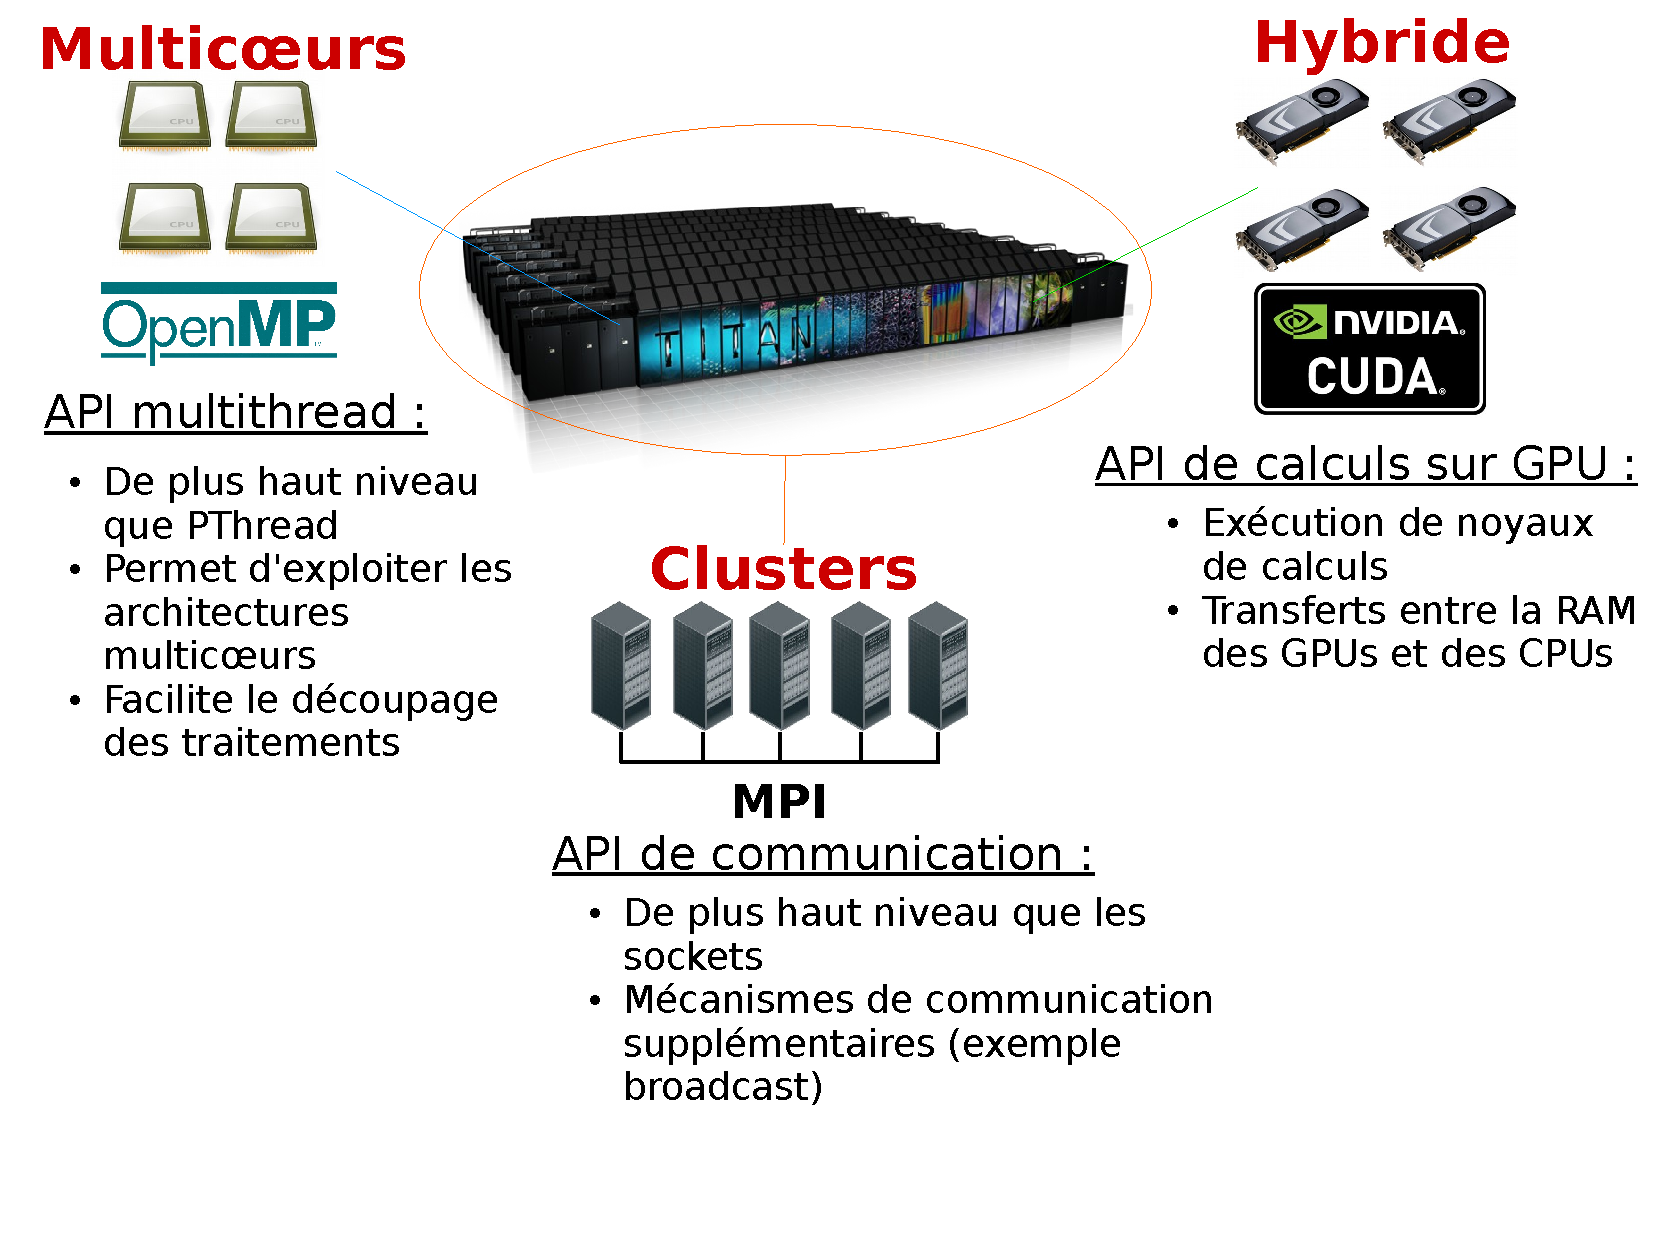
\includegraphics[width=\linewidth]{./Slides/Archi.pdf}
\end{figure}
\end{frame}

\begin{frame}[label=sec-2-2]{Limites des approches classiques}
\begin{itemize}
\item Utiliser \alert{plusieurs paradigmes} $\leadsto$ \alert{programmation complexe}
\item Exemple pour exploiter efficacement un GPU sur \alert{un seul noeud}:
\begin{itemize}
\item \alert{transférer données} du CPU au GPU,
\item \alert{lancer le calcul} sur le GPU
\item \alert{gérer synchronisation} pendant attente résultat
\item \alert{occuper} CPU
\item \alert{récupérer} résultat.
\end{itemize}
\item Et avec \alert{plusieurs noeuds}?
\item \alert{Statique}, système réglé comme un horloge $\leadsto$ pas portable.
\item Solution: \alert{Dynamique} mais presque \alert{impossible avec APIs classiques}.
\end{itemize}
\end{frame}
\begin{frame}[label=sec-2-3]{Nouvelle approche: Paradigme de tâches}
\begin{columns}
  \begin{column}{.55\linewidth}
\begin{itemize}
\item Nouvelle abstraction: les tâches
\begin{itemize}
\item \alert{Plus besoin de se soucier de la ressource} sur laquelle le
traitement est effectué.
\item Exprimer calcul en \alert{graphe de tâches} $\leadsto$ système dynamique
plus simple.
\end{itemize}
\end{itemize}

  \end{column}
  \begin{column}{.35\linewidth}
    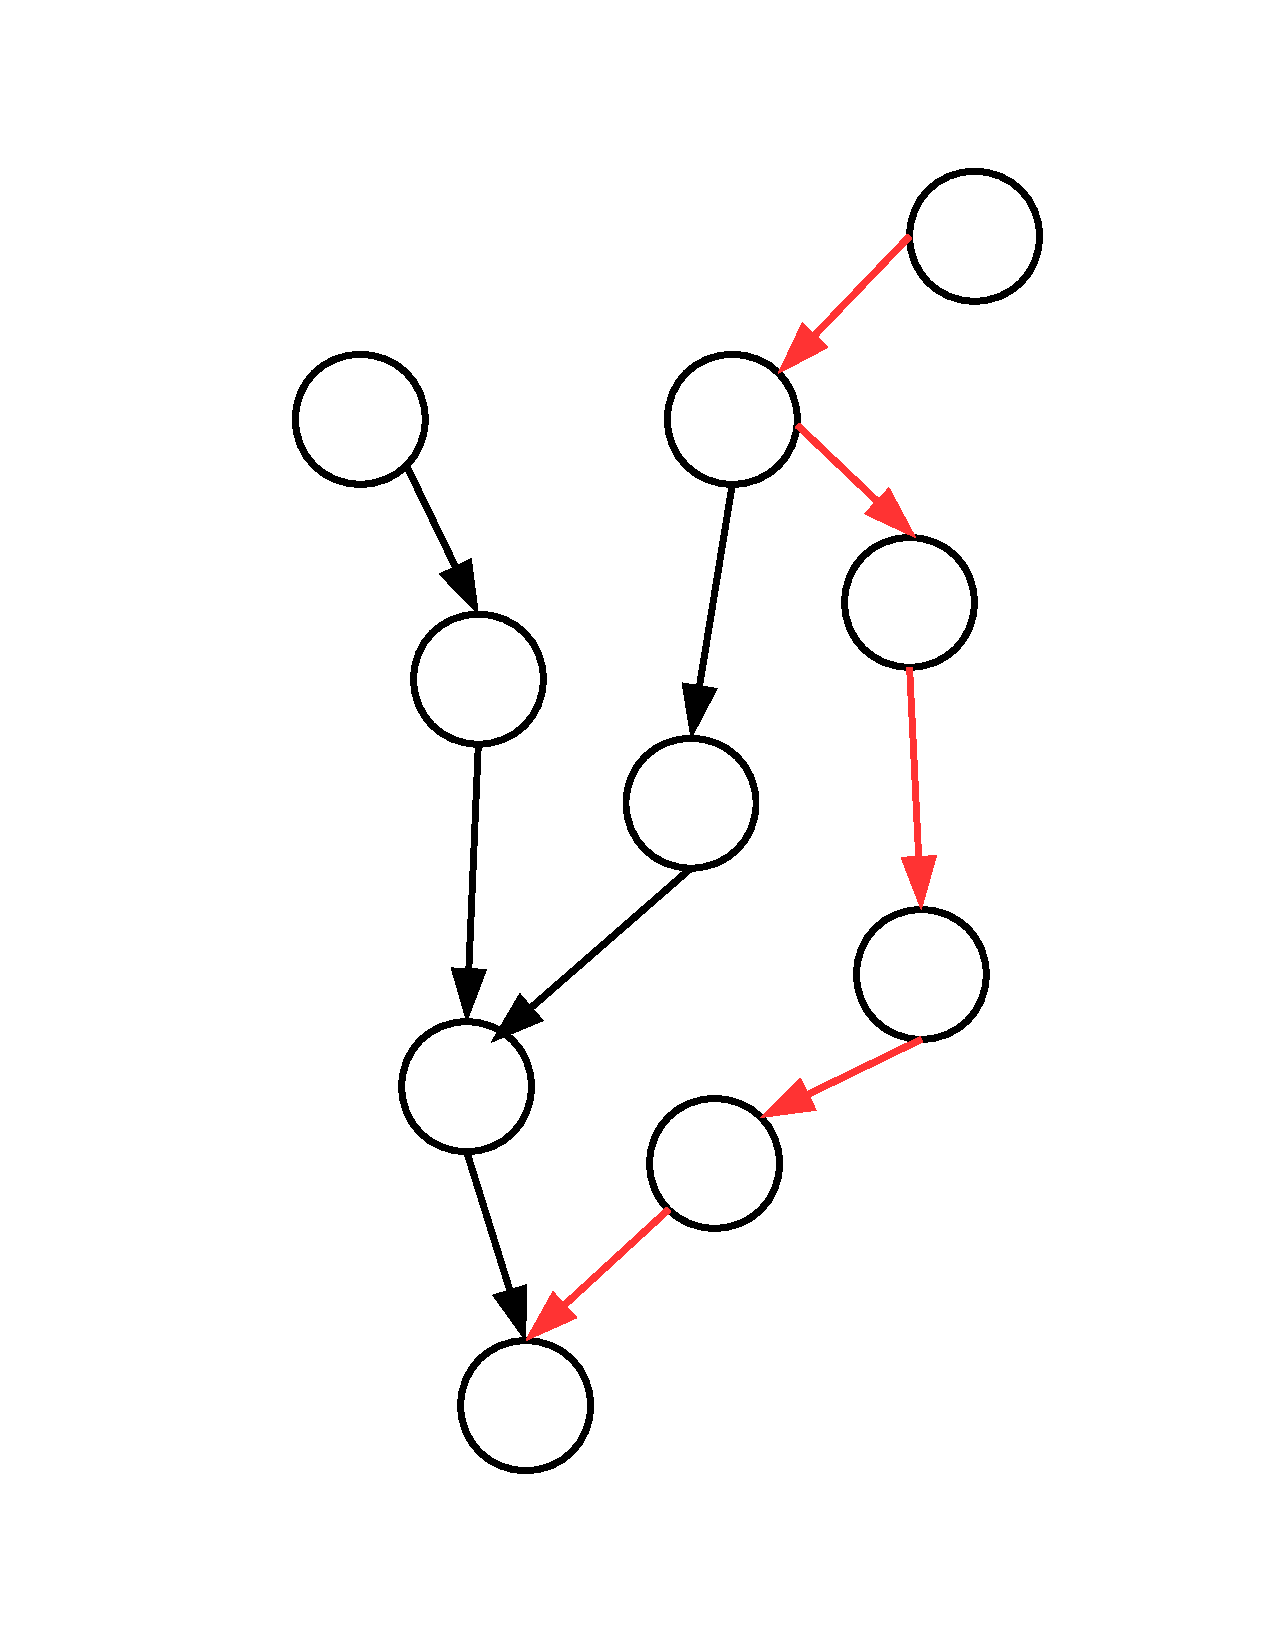
\includegraphics[width=.45\linewidth]{img/task_graph.jpg}%
  \end{column}
\end{columns}

\begin{itemize}
\item Librairie StarPU:
\begin{itemize}
\item Système \alert{runtime}
\item basé sur le paradigme de tâches $\leadsto$ graphe de dépendances.
\item Ordonnancemment \alert{dynamique et opportuniste}.
\end{itemize}
\item Problèmatique : Performances difficiles à évaluer
\begin{itemize}
\item Configuration \alert{runtinme}, heuristique, politique ordonnancement.
\item Configuration \alert{application}, découpage des tâches.
\end{itemize}
\end{itemize}
\end{frame}
\section{État de l'art}
\label{sec-3}
\begin{frame}[label=sec-3-1]{Test sur systèmes réels}
\begin{itemize}
\item Exécution réelle sur la plateforme cible $\leadsto$ \alert{coûteux}
\item Exéuction \alert{non déterministe} nécessite de réaliser beaucoup
d'expériences $\leadsto$ extrapolations difficiles.
\end{itemize}
\end{frame}
\begin{frame}[label=sec-3-2]{Simulation}
\begin{block}{Généralités}
\begin{itemize}
\item Utilisation de \alert{modèles} pour \alert{prédire} comportements.
\item Permet s'affranchir de la plateforme $\leadsto$ peu coûteux.
\item Contrôle paramètres $\leadsto$ \alert{systèmes déterministes}.
\item Extrapolation simplifiée.
\item Exécution plus courte.
\end{itemize}
\end{block}

\begin{block}{Simulation par rejeu de trace}
Exécution post-mortem: pas adapté ici car \alert{flot de contrôle non
déterministe}.
\end{block}
\begin{block}{Hybride simulation / émulation}
\begin{itemize}
\item Simuler plateforme et OS.
\item Emuler de l'application.
\end{itemize}
\end{block}
\end{frame}
\section{Analyse du problème}
\label{sec-4}
\begin{frame}[label=sec-4-1]{SimGrid: Généralités}
\begin{figure}
\centering
\vspace{-4.5mm}
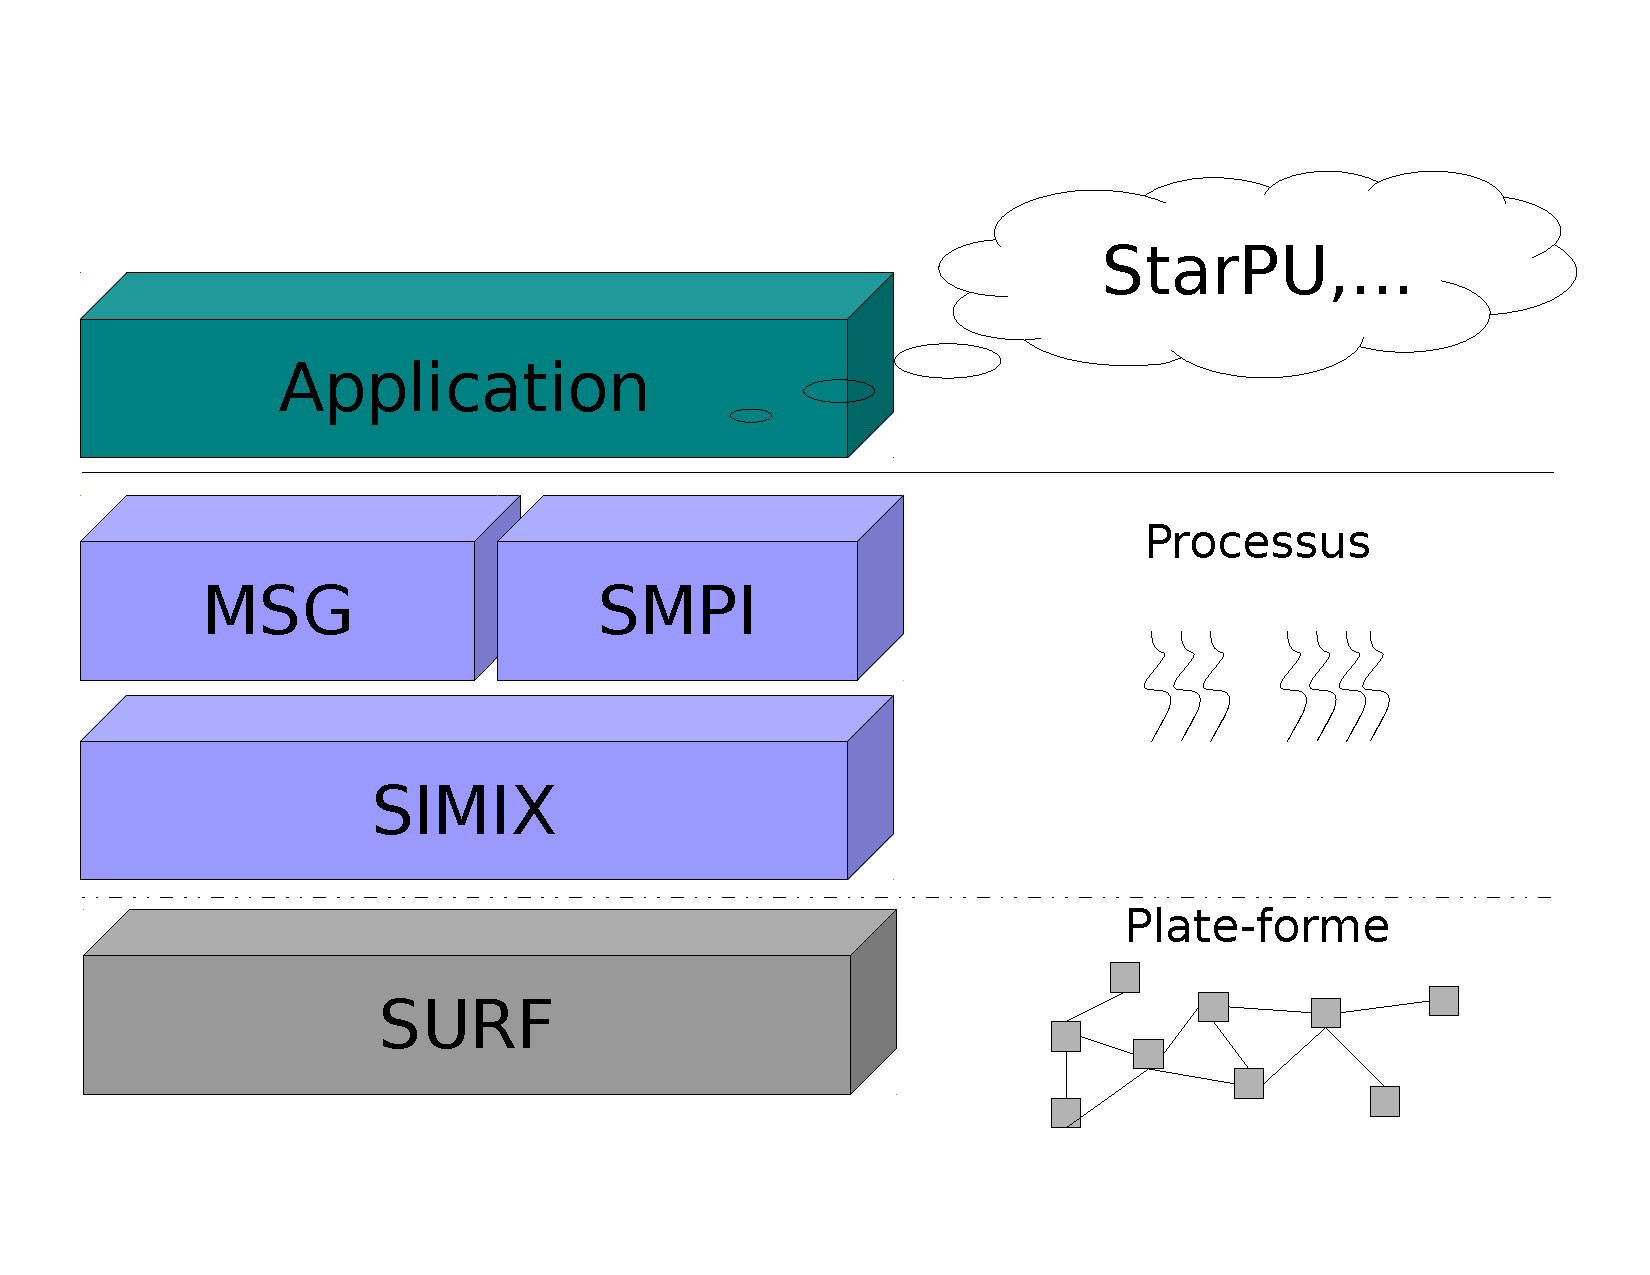
\includegraphics[width=\linewidth]{../Img/Simgrid.pdf}
\end{figure}
\end{frame}

\begin{frame}[label=sec-4-2]{Construction de l'application MPI simulée}
\begin{figure}
\centering
\vspace{-4.5mm}
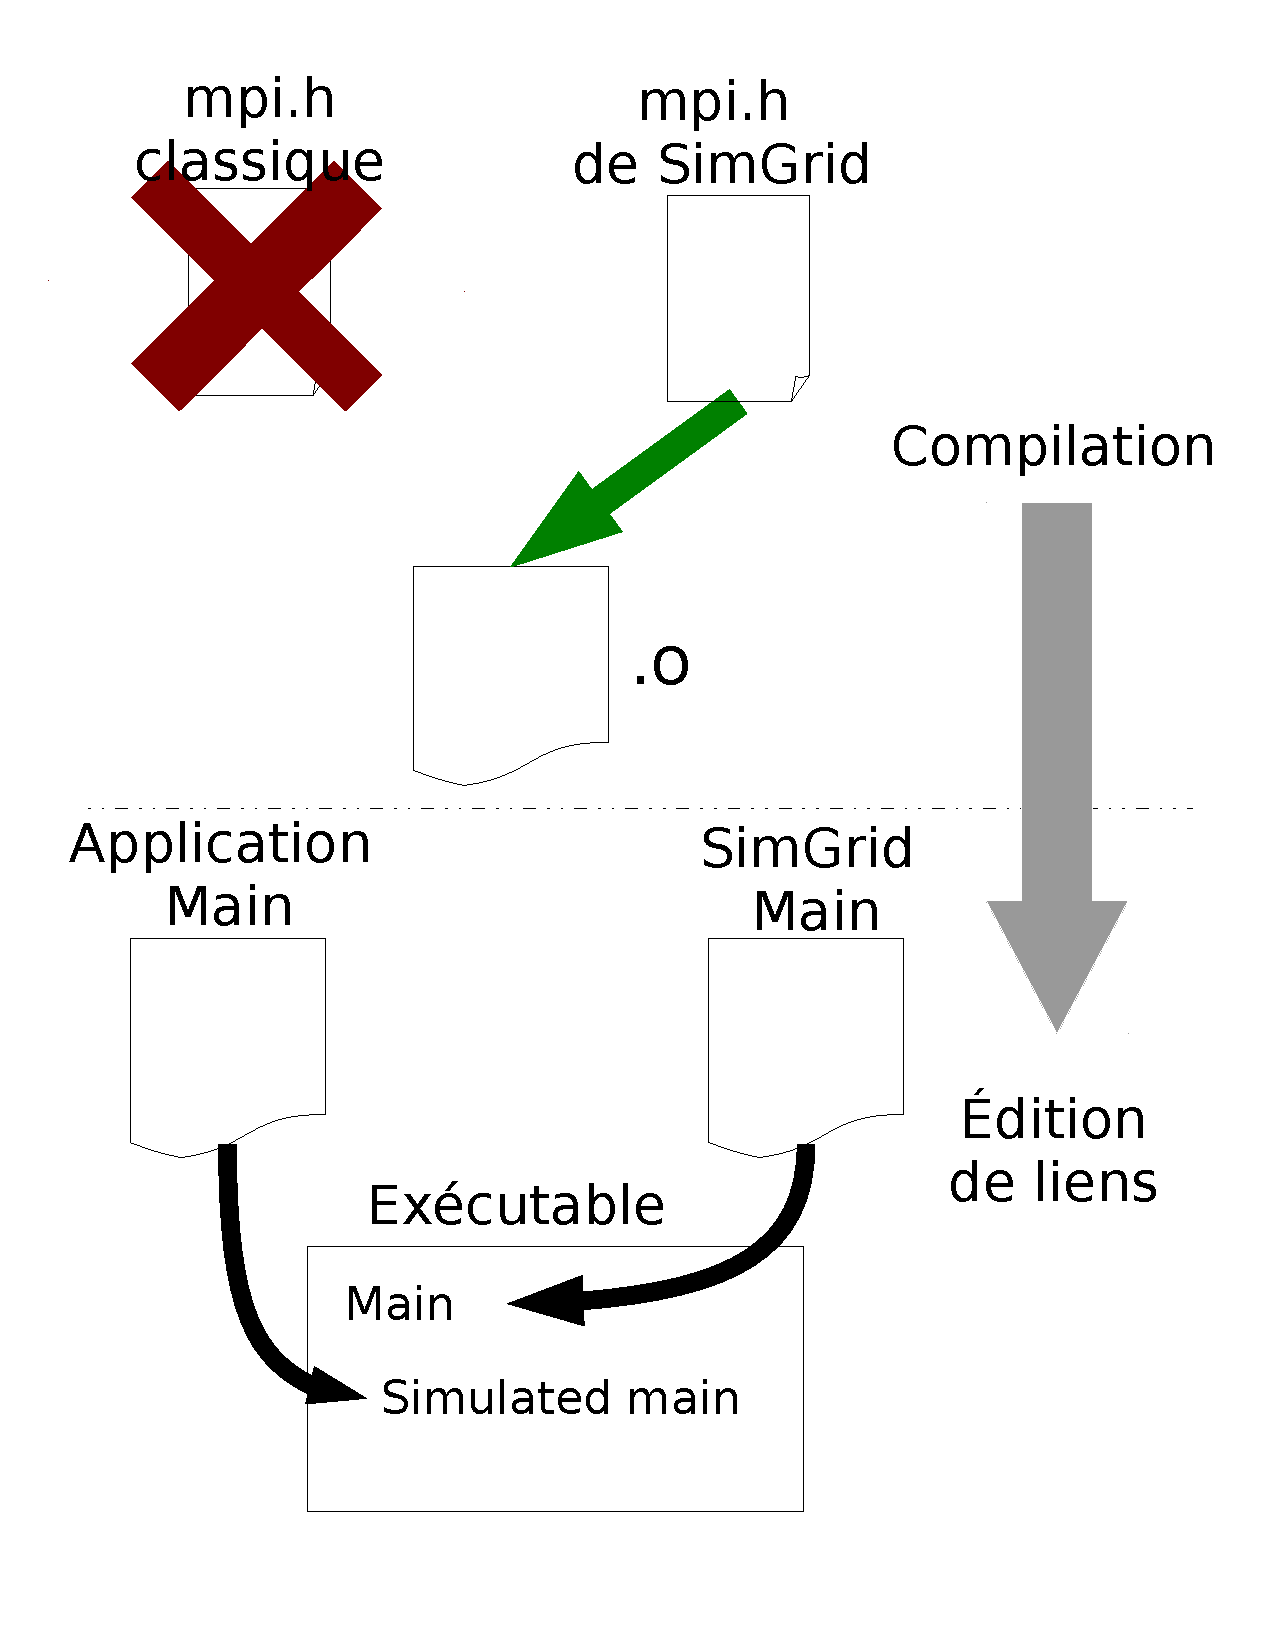
\includegraphics[width=.45\linewidth]{../Img/Compile.pdf}
\end{figure}
\end{frame}

\begin{frame}[label=sec-4-3]{Privatisation segment data}
\begin{columns}
  \begin{column}{.45\linewidth}
\begin{itemize}
\item Dans SimGrid les \alert{processus} sont \alert{modélisés par des threads} $\leadsto$
  espace adressage partagé.
\item Mécanisme de privatisation: \alert{ségment virtuel} (mmap)
\end{itemize}


  \end{column}
  \begin{column}{.45\linewidth}
    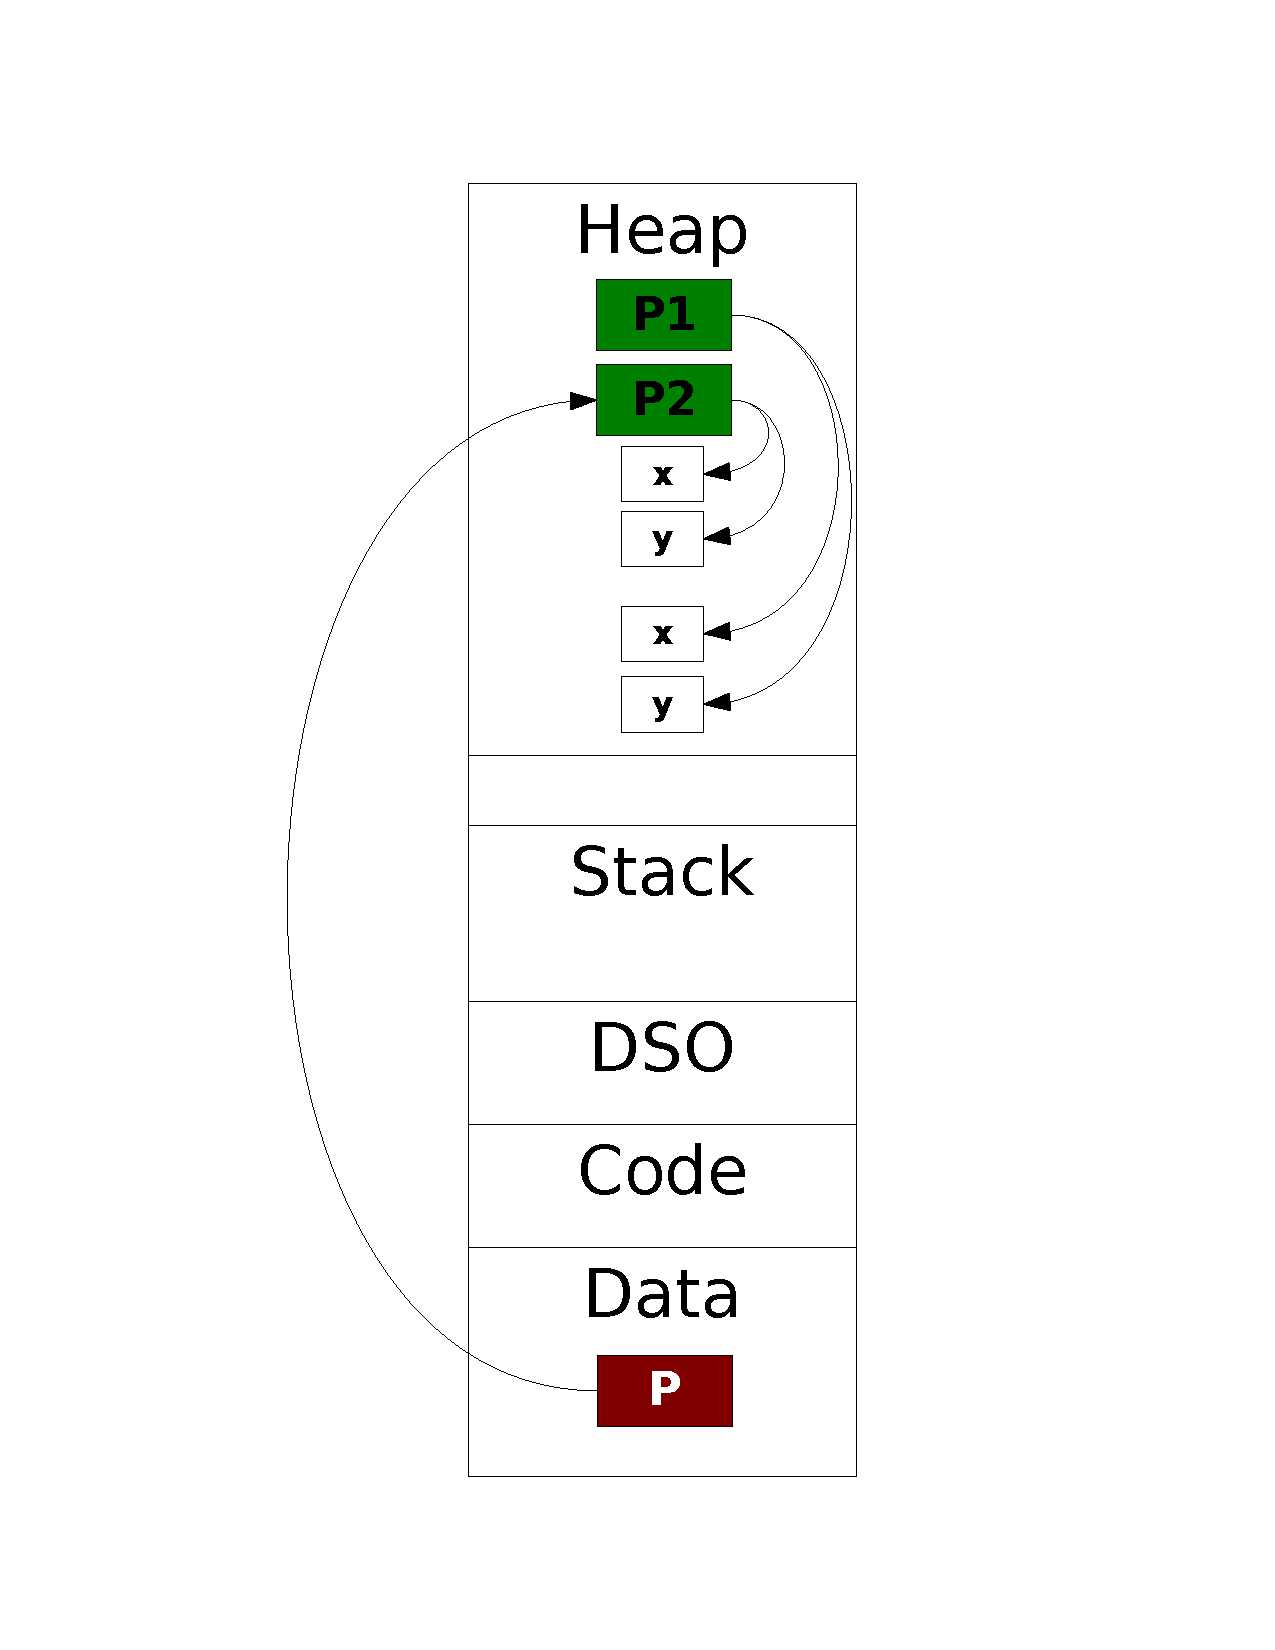
\includegraphics[width=\linewidth]{../Img/Memoire.pdf}
  \end{column}
\end{columns}
\end{frame}

\begin{frame}[label=sec-4-4]{StarPU MSG}
\begin{itemize}
\item Basé sur \alert{MSG} car \alert{modèle de performance plus proche} (communications,
environnement mémoire partagé), CPUs GPUs.
\item Simulation: calculs, allocations mémoire des tâches, transfert
CUDA.
\end{itemize}
\end{frame}
\begin{frame}[label=sec-4-5]{StarPU SMPI: Difficultés de mise en oeuvre}
\begin{itemize}
\item Besoin de \alert{2 modèles de performances} différents à la fois:
\begin{itemize}
\item \alert{MSG} Intra noeuds $\leadsto$ mémoire partagée $\leadsto$ partage.
\item \alert{SMPI} extra noeuds $\leadsto$ mémoire distribuée $\leadsto$
   privatisation.
\end{itemize}
\item MSG et SMPI normalement pas utilisés ensemble $\leadsto$ initialiser
correctement les 2.
\end{itemize}
\begin{columns}[]
  \begin{column}{.55\linewidth}
\begin{itemize}
\item Problème des librairies dynamiques.
\end{itemize}
  \end{column}
  \begin{column}{.35\linewidth}
 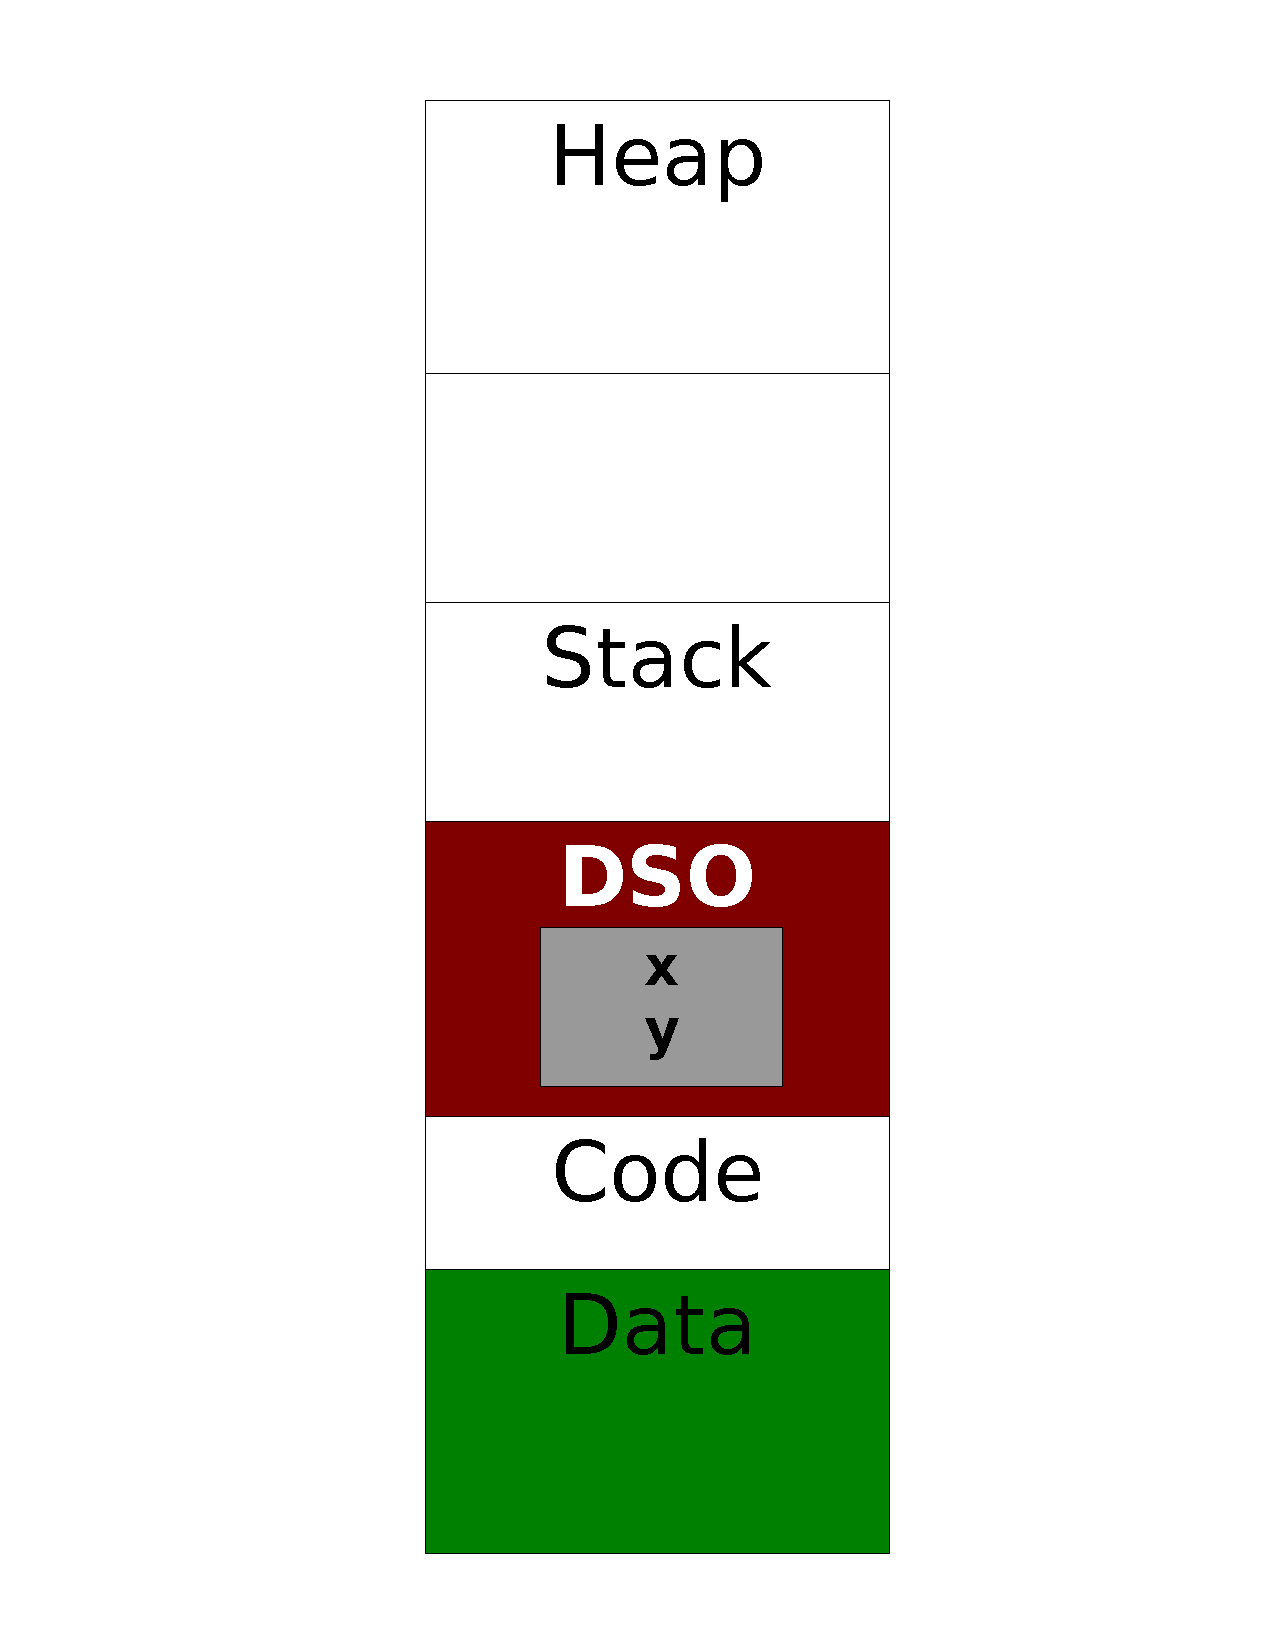
\includegraphics[width=.7\linewidth]{../Img/Dyn.pdf}
  \end{column}
\end{columns}
\end{frame}



\section{Méthodologie}
\label{sec-5}
\section{Contribution}
\label{sec-6}
\section{Validation}
\label{sec-7}
\section{Conclusion}
\label{sec-8}
% Emacs 24.5.1 (Org mode 8.2.10)
\end{document}